% Created by tikzDevice version 0.12.6 on 2026-08-08 12:11:58
% !TEX encoding = UTF-8 Unicode
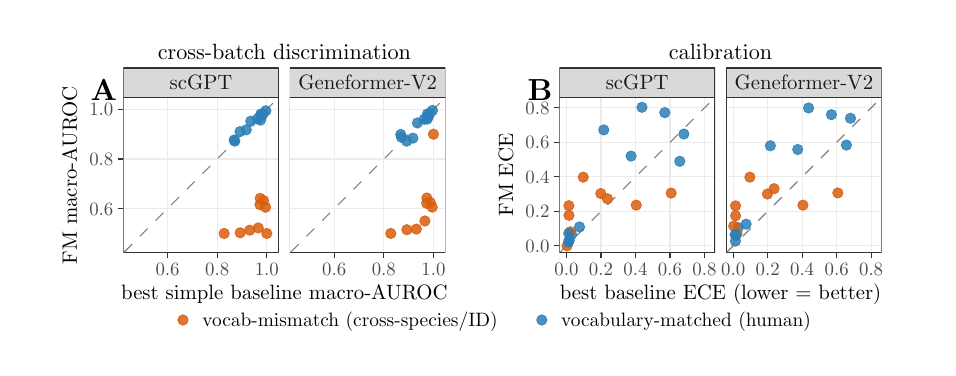
\begin{tikzpicture}[x=1pt,y=1pt]
\definecolor{fillColor}{RGB}{255,255,255}
\path[use as bounding box,fill=fillColor,fill opacity=0.00] (0,0) rectangle (325.21,115.63);
\begin{scope}
\path[clip] (  0.00,  0.00) rectangle (325.21,115.63);
\definecolor{drawColor}{RGB}{255,255,255}
\definecolor{fillColor}{RGB}{255,255,255}

\path[draw=drawColor,line width= 0.4pt,line join=round,line cap=round,fill=fillColor] (  0.00,  0.00) rectangle (325.21,115.63);
\end{scope}
\begin{scope}
\path[clip] (  4.00,  3.00) rectangle (161.61,112.63);
\definecolor{drawColor}{RGB}{255,255,255}
\definecolor{fillColor}{RGB}{255,255,255}

\path[draw=drawColor,line width= 0.4pt,line join=round,line cap=round,fill=fillColor] (  4.00,  3.00) rectangle (161.61,112.63);
\end{scope}
\begin{scope}
\path[clip] (161.61,  3.00) rectangle (319.21,112.63);
\definecolor{drawColor}{RGB}{255,255,255}
\definecolor{fillColor}{RGB}{255,255,255}

\path[draw=drawColor,line width= 0.4pt,line join=round,line cap=round,fill=fillColor] (161.61,  3.00) rectangle (319.21,112.63);
\end{scope}
\begin{scope}
\path[clip] ( 34.54, 34.23) rectangle ( 90.76, 90.44);
\definecolor{fillColor}{RGB}{255,255,255}

\path[fill=fillColor] ( 34.54, 34.23) rectangle ( 90.76, 90.44);
\definecolor{drawColor}{gray}{0.92}

\path[draw=drawColor,line width= 0.4pt,line join=round] ( 34.54, 50.23) --
	( 90.76, 50.23);

\path[draw=drawColor,line width= 0.4pt,line join=round] ( 34.54, 68.16) --
	( 90.76, 68.16);

\path[draw=drawColor,line width= 0.4pt,line join=round] ( 34.54, 86.10) --
	( 90.76, 86.10);

\path[draw=drawColor,line width= 0.4pt,line join=round] ( 50.55, 34.23) --
	( 50.55, 90.44);

\path[draw=drawColor,line width= 0.4pt,line join=round] ( 68.48, 34.23) --
	( 68.48, 90.44);

\path[draw=drawColor,line width= 0.4pt,line join=round] ( 86.41, 34.23) --
	( 86.41, 90.44);
\definecolor{drawColor}{gray}{0.50}

\path[draw=drawColor,line width= 0.4pt,dash pattern=on 4pt off 4pt ,line join=round] (-21.67,-21.99) -- (146.97,146.66);
\definecolor{drawColor}{RGB}{44,127,184}
\definecolor{fillColor}{RGB}{44,127,184}

\path[draw=drawColor,draw opacity=0.85,line width= 0.3pt,line join=round,line cap=round,fill=fillColor,fill opacity=0.85] ( 84.55, 83.74) circle (  1.87);

\path[draw=drawColor,draw opacity=0.85,line width= 0.3pt,line join=round,line cap=round,fill=fillColor,fill opacity=0.85] ( 74.85, 74.62) circle (  1.87);
\definecolor{drawColor}{RGB}{217,95,14}
\definecolor{fillColor}{RGB}{217,95,14}

\path[draw=drawColor,draw opacity=0.85,line width= 0.3pt,line join=round,line cap=round,fill=fillColor,fill opacity=0.85] ( 83.92, 51.68) circle (  1.87);
\definecolor{drawColor}{RGB}{44,127,184}
\definecolor{fillColor}{RGB}{44,127,184}

\path[draw=drawColor,draw opacity=0.85,line width= 0.3pt,line join=round,line cap=round,fill=fillColor,fill opacity=0.85] ( 74.58, 75.03) circle (  1.87);

\path[draw=drawColor,draw opacity=0.85,line width= 0.3pt,line join=round,line cap=round,fill=fillColor,fill opacity=0.85] ( 78.99, 78.71) circle (  1.87);
\definecolor{drawColor}{RGB}{217,95,14}
\definecolor{fillColor}{RGB}{217,95,14}

\path[draw=drawColor,draw opacity=0.85,line width= 0.3pt,line join=round,line cap=round,fill=fillColor,fill opacity=0.85] ( 84.02, 53.96) circle (  1.87);
\definecolor{drawColor}{RGB}{44,127,184}
\definecolor{fillColor}{RGB}{44,127,184}

\path[draw=drawColor,draw opacity=0.85,line width= 0.3pt,line join=round,line cap=round,fill=fillColor,fill opacity=0.85] ( 84.13, 82.21) circle (  1.87);
\definecolor{drawColor}{RGB}{217,95,14}
\definecolor{fillColor}{RGB}{217,95,14}

\path[draw=drawColor,draw opacity=0.85,line width= 0.3pt,line join=round,line cap=round,fill=fillColor,fill opacity=0.85] ( 85.27, 53.12) circle (  1.87);
\definecolor{drawColor}{RGB}{44,127,184}
\definecolor{fillColor}{RGB}{44,127,184}

\path[draw=drawColor,draw opacity=0.85,line width= 0.3pt,line join=round,line cap=round,fill=fillColor,fill opacity=0.85] ( 80.61, 81.82) circle (  1.87);

\path[draw=drawColor,draw opacity=0.85,line width= 0.3pt,line join=round,line cap=round,fill=fillColor,fill opacity=0.85] ( 76.72, 78.07) circle (  1.87);

\path[draw=drawColor,draw opacity=0.85,line width= 0.3pt,line join=round,line cap=round,fill=fillColor,fill opacity=0.85] ( 84.24, 84.40) circle (  1.87);

\path[draw=drawColor,draw opacity=0.85,line width= 0.3pt,line join=round,line cap=round,fill=fillColor,fill opacity=0.85] ( 83.08, 82.67) circle (  1.87);
\definecolor{drawColor}{RGB}{217,95,14}
\definecolor{fillColor}{RGB}{217,95,14}

\path[draw=drawColor,draw opacity=0.85,line width= 0.3pt,line join=round,line cap=round,fill=fillColor,fill opacity=0.85] ( 86.41, 41.27) circle (  1.87);

\path[draw=drawColor,draw opacity=0.85,line width= 0.3pt,line join=round,line cap=round,fill=fillColor,fill opacity=0.85] ( 71.00, 41.27) circle (  1.87);

\path[draw=drawColor,draw opacity=0.85,line width= 0.3pt,line join=round,line cap=round,fill=fillColor,fill opacity=0.85] ( 83.32, 43.26) circle (  1.87);
\definecolor{drawColor}{RGB}{44,127,184}
\definecolor{fillColor}{RGB}{44,127,184}

\path[draw=drawColor,draw opacity=0.85,line width= 0.3pt,line join=round,line cap=round,fill=fillColor,fill opacity=0.85] ( 86.07, 85.62) circle (  1.87);
\definecolor{drawColor}{RGB}{217,95,14}
\definecolor{fillColor}{RGB}{217,95,14}

\path[draw=drawColor,draw opacity=0.85,line width= 0.3pt,line join=round,line cap=round,fill=fillColor,fill opacity=0.85] ( 80.25, 42.45) circle (  1.87);
\definecolor{drawColor}{RGB}{44,127,184}
\definecolor{fillColor}{RGB}{44,127,184}

\path[draw=drawColor,draw opacity=0.85,line width= 0.3pt,line join=round,line cap=round,fill=fillColor,fill opacity=0.85] ( 85.13, 84.57) circle (  1.87);
\definecolor{drawColor}{RGB}{217,95,14}
\definecolor{fillColor}{RGB}{217,95,14}

\path[draw=drawColor,draw opacity=0.85,line width= 0.3pt,line join=round,line cap=round,fill=fillColor,fill opacity=0.85] ( 85.96, 50.73) circle (  1.87);

\path[draw=drawColor,draw opacity=0.85,line width= 0.3pt,line join=round,line cap=round,fill=fillColor,fill opacity=0.85] ( 76.80, 41.52) circle (  1.87);
\definecolor{drawColor}{gray}{0.20}

\path[draw=drawColor,line width= 0.4pt,line join=round,line cap=round] ( 34.54, 34.23) rectangle ( 90.76, 90.44);
\end{scope}
\begin{scope}
\path[clip] ( 94.76, 34.23) rectangle (150.97, 90.44);
\definecolor{fillColor}{RGB}{255,255,255}

\path[fill=fillColor] ( 94.76, 34.23) rectangle (150.97, 90.44);
\definecolor{drawColor}{gray}{0.92}

\path[draw=drawColor,line width= 0.4pt,line join=round] ( 94.76, 50.23) --
	(150.97, 50.23);

\path[draw=drawColor,line width= 0.4pt,line join=round] ( 94.76, 68.16) --
	(150.97, 68.16);

\path[draw=drawColor,line width= 0.4pt,line join=round] ( 94.76, 86.10) --
	(150.97, 86.10);

\path[draw=drawColor,line width= 0.4pt,line join=round] (110.76, 34.23) --
	(110.76, 90.44);

\path[draw=drawColor,line width= 0.4pt,line join=round] (128.69, 34.23) --
	(128.69, 90.44);

\path[draw=drawColor,line width= 0.4pt,line join=round] (146.63, 34.23) --
	(146.63, 90.44);
\definecolor{drawColor}{gray}{0.50}

\path[draw=drawColor,line width= 0.4pt,dash pattern=on 4pt off 4pt ,line join=round] ( 38.54,-21.99) -- (207.19,146.66);
\definecolor{drawColor}{RGB}{44,127,184}
\definecolor{fillColor}{RGB}{44,127,184}

\path[draw=drawColor,draw opacity=0.85,line width= 0.3pt,line join=round,line cap=round,fill=fillColor,fill opacity=0.85] (144.77, 83.50) circle (  1.87);

\path[draw=drawColor,draw opacity=0.85,line width= 0.3pt,line join=round,line cap=round,fill=fillColor,fill opacity=0.85] (135.06, 76.06) circle (  1.87);
\definecolor{drawColor}{RGB}{217,95,14}
\definecolor{fillColor}{RGB}{217,95,14}

\path[draw=drawColor,draw opacity=0.85,line width= 0.3pt,line join=round,line cap=round,fill=fillColor,fill opacity=0.85] (144.14, 52.18) circle (  1.87);
\definecolor{drawColor}{RGB}{44,127,184}
\definecolor{fillColor}{RGB}{44,127,184}

\path[draw=drawColor,draw opacity=0.85,line width= 0.3pt,line join=round,line cap=round,fill=fillColor,fill opacity=0.85] (134.80, 77.04) circle (  1.87);

\path[draw=drawColor,draw opacity=0.85,line width= 0.3pt,line join=round,line cap=round,fill=fillColor,fill opacity=0.85] (139.20, 75.71) circle (  1.87);
\definecolor{drawColor}{RGB}{217,95,14}
\definecolor{fillColor}{RGB}{217,95,14}

\path[draw=drawColor,draw opacity=0.85,line width= 0.3pt,line join=round,line cap=round,fill=fillColor,fill opacity=0.85] (144.24, 54.07) circle (  1.87);
\definecolor{drawColor}{RGB}{44,127,184}
\definecolor{fillColor}{RGB}{44,127,184}

\path[draw=drawColor,draw opacity=0.85,line width= 0.3pt,line join=round,line cap=round,fill=fillColor,fill opacity=0.85] (144.35, 82.57) circle (  1.87);
\definecolor{drawColor}{RGB}{217,95,14}
\definecolor{fillColor}{RGB}{217,95,14}

\path[draw=drawColor,draw opacity=0.85,line width= 0.3pt,line join=round,line cap=round,fill=fillColor,fill opacity=0.85] (145.48, 52.46) circle (  1.87);
\definecolor{drawColor}{RGB}{44,127,184}
\definecolor{fillColor}{RGB}{44,127,184}

\path[draw=drawColor,draw opacity=0.85,line width= 0.3pt,line join=round,line cap=round,fill=fillColor,fill opacity=0.85] (140.82, 81.20) circle (  1.87);

\path[draw=drawColor,draw opacity=0.85,line width= 0.3pt,line join=round,line cap=round,fill=fillColor,fill opacity=0.85] (136.94, 74.62) circle (  1.87);

\path[draw=drawColor,draw opacity=0.85,line width= 0.3pt,line join=round,line cap=round,fill=fillColor,fill opacity=0.85] (144.46, 84.47) circle (  1.87);

\path[draw=drawColor,draw opacity=0.85,line width= 0.3pt,line join=round,line cap=round,fill=fillColor,fill opacity=0.85] (143.29, 82.53) circle (  1.87);
\definecolor{drawColor}{RGB}{217,95,14}
\definecolor{fillColor}{RGB}{217,95,14}

\path[draw=drawColor,draw opacity=0.85,line width= 0.3pt,line join=round,line cap=round,fill=fillColor,fill opacity=0.85] (146.63, 77.13) circle (  1.87);

\path[draw=drawColor,draw opacity=0.85,line width= 0.3pt,line join=round,line cap=round,fill=fillColor,fill opacity=0.85] (131.21, 41.27) circle (  1.87);

\path[draw=drawColor,draw opacity=0.85,line width= 0.3pt,line join=round,line cap=round,fill=fillColor,fill opacity=0.85] (143.54, 45.77) circle (  1.87);
\definecolor{drawColor}{RGB}{44,127,184}
\definecolor{fillColor}{RGB}{44,127,184}

\path[draw=drawColor,draw opacity=0.85,line width= 0.3pt,line join=round,line cap=round,fill=fillColor,fill opacity=0.85] (146.29, 85.74) circle (  1.87);
\definecolor{drawColor}{RGB}{217,95,14}
\definecolor{fillColor}{RGB}{217,95,14}

\path[draw=drawColor,draw opacity=0.85,line width= 0.3pt,line join=round,line cap=round,fill=fillColor,fill opacity=0.85] (140.46, 42.85) circle (  1.87);
\definecolor{drawColor}{RGB}{44,127,184}
\definecolor{fillColor}{RGB}{44,127,184}

\path[draw=drawColor,draw opacity=0.85,line width= 0.3pt,line join=round,line cap=round,fill=fillColor,fill opacity=0.85] (145.35, 84.69) circle (  1.87);
\definecolor{drawColor}{RGB}{217,95,14}
\definecolor{fillColor}{RGB}{217,95,14}

\path[draw=drawColor,draw opacity=0.85,line width= 0.3pt,line join=round,line cap=round,fill=fillColor,fill opacity=0.85] (146.18, 50.77) circle (  1.87);

\path[draw=drawColor,draw opacity=0.85,line width= 0.3pt,line join=round,line cap=round,fill=fillColor,fill opacity=0.85] (137.02, 42.62) circle (  1.87);
\definecolor{drawColor}{gray}{0.20}

\path[draw=drawColor,line width= 0.4pt,line join=round,line cap=round] ( 94.76, 34.23) rectangle (150.97, 90.44);
\end{scope}
\begin{scope}
\path[clip] (  0.00,  0.00) rectangle (325.21,115.63);
\definecolor{drawColor}{RGB}{0,0,0}

\node[text=drawColor,anchor=base,inner sep=0pt, outer sep=0pt, scale=  1.10] at ( 27.56, 89.46) {\bfseries A};
\end{scope}
\begin{scope}
\path[clip] (  0.00,  0.00) rectangle (325.21,115.63);
\definecolor{drawColor}{gray}{0.30}

\node[text=drawColor,anchor=base east,inner sep=0pt, outer sep=0pt, scale=  0.68] at ( 30.94, 47.89) {0.6};

\node[text=drawColor,anchor=base east,inner sep=0pt, outer sep=0pt, scale=  0.68] at ( 30.94, 65.82) {0.8};

\node[text=drawColor,anchor=base east,inner sep=0pt, outer sep=0pt, scale=  0.68] at ( 30.94, 83.75) {1.0};
\end{scope}
\begin{scope}
\path[clip] (  0.00,  0.00) rectangle (325.21,115.63);
\definecolor{drawColor}{gray}{0.20}

\path[draw=drawColor,line width= 0.4pt,line join=round] ( 32.54, 50.23) --
	( 34.54, 50.23);

\path[draw=drawColor,line width= 0.4pt,line join=round] ( 32.54, 68.16) --
	( 34.54, 68.16);

\path[draw=drawColor,line width= 0.4pt,line join=round] ( 32.54, 86.10) --
	( 34.54, 86.10);
\end{scope}
\begin{scope}
\path[clip] (  0.00,  0.00) rectangle (325.21,115.63);
\definecolor{drawColor}{RGB}{0,0,0}

\node[text=drawColor,rotate= 90.00,anchor=base,inner sep=0pt, outer sep=0pt, scale=  0.75] at ( 17.80, 62.34) {FM macro-AUROC};
\end{scope}
\begin{scope}
\path[clip] ( 34.54, 90.44) rectangle ( 90.76,101.07);
\definecolor{drawColor}{gray}{0.20}
\definecolor{fillColor}{gray}{0.85}

\path[draw=drawColor,line width= 0.4pt,line join=round,line cap=round,fill=fillColor] ( 34.54, 90.44) rectangle ( 90.76,101.07);
\definecolor{drawColor}{gray}{0.10}

\node[text=drawColor,anchor=base,inner sep=0pt, outer sep=0pt, scale=  0.75] at ( 62.65, 93.17) {scGPT};
\end{scope}
\begin{scope}
\path[clip] ( 94.76, 90.44) rectangle (150.97,101.07);
\definecolor{drawColor}{gray}{0.20}
\definecolor{fillColor}{gray}{0.85}

\path[draw=drawColor,line width= 0.4pt,line join=round,line cap=round,fill=fillColor] ( 94.76, 90.44) rectangle (150.97,101.07);
\definecolor{drawColor}{gray}{0.10}

\node[text=drawColor,anchor=base,inner sep=0pt, outer sep=0pt, scale=  0.75] at (122.87, 93.17) {Geneformer-V2};
\end{scope}
\begin{scope}
\path[clip] (  0.00,  0.00) rectangle (325.21,115.63);
\definecolor{drawColor}{gray}{0.20}

\path[draw=drawColor,line width= 0.4pt,line join=round] ( 50.55, 32.23) --
	( 50.55, 34.23);

\path[draw=drawColor,line width= 0.4pt,line join=round] ( 68.48, 32.23) --
	( 68.48, 34.23);

\path[draw=drawColor,line width= 0.4pt,line join=round] ( 86.41, 32.23) --
	( 86.41, 34.23);
\end{scope}
\begin{scope}
\path[clip] (  0.00,  0.00) rectangle (325.21,115.63);
\definecolor{drawColor}{gray}{0.30}

\node[text=drawColor,anchor=base,inner sep=0pt, outer sep=0pt, scale=  0.68] at ( 50.55, 25.95) {0.6};

\node[text=drawColor,anchor=base,inner sep=0pt, outer sep=0pt, scale=  0.68] at ( 68.48, 25.95) {0.8};

\node[text=drawColor,anchor=base,inner sep=0pt, outer sep=0pt, scale=  0.68] at ( 86.41, 25.95) {1.0};
\end{scope}
\begin{scope}
\path[clip] (  0.00,  0.00) rectangle (325.21,115.63);
\definecolor{drawColor}{gray}{0.20}

\path[draw=drawColor,line width= 0.4pt,line join=round] (110.76, 32.23) --
	(110.76, 34.23);

\path[draw=drawColor,line width= 0.4pt,line join=round] (128.69, 32.23) --
	(128.69, 34.23);

\path[draw=drawColor,line width= 0.4pt,line join=round] (146.63, 32.23) --
	(146.63, 34.23);
\end{scope}
\begin{scope}
\path[clip] (  0.00,  0.00) rectangle (325.21,115.63);
\definecolor{drawColor}{gray}{0.30}

\node[text=drawColor,anchor=base,inner sep=0pt, outer sep=0pt, scale=  0.68] at (110.76, 25.95) {0.6};

\node[text=drawColor,anchor=base,inner sep=0pt, outer sep=0pt, scale=  0.68] at (128.69, 25.95) {0.8};

\node[text=drawColor,anchor=base,inner sep=0pt, outer sep=0pt, scale=  0.68] at (146.63, 25.95) {1.0};
\end{scope}
\begin{scope}
\path[clip] (  0.00,  0.00) rectangle (325.21,115.63);
\definecolor{drawColor}{RGB}{0,0,0}

\node[text=drawColor,anchor=base,inner sep=0pt, outer sep=0pt, scale=  0.75] at ( 92.76, 17.46) {best simple baseline macro-AUROC};
\end{scope}
\begin{scope}
\path[clip] (  0.00,  0.00) rectangle (325.21,115.63);
\definecolor{drawColor}{RGB}{0,0,0}

\node[text=drawColor,anchor=base,inner sep=0pt, outer sep=0pt, scale=  0.80] at ( 92.76,104.12) {cross-batch discrimination};
\end{scope}
\begin{scope}
\path[clip] (192.15, 34.23) rectangle (248.37, 90.44);
\definecolor{fillColor}{RGB}{255,255,255}

\path[fill=fillColor] (192.15, 34.23) rectangle (248.37, 90.44);
\definecolor{drawColor}{gray}{0.92}

\path[draw=drawColor,line width= 0.4pt,line join=round] (192.15, 36.78) --
	(248.37, 36.78);

\path[draw=drawColor,line width= 0.4pt,line join=round] (192.15, 49.25) --
	(248.37, 49.25);

\path[draw=drawColor,line width= 0.4pt,line join=round] (192.15, 61.71) --
	(248.37, 61.71);

\path[draw=drawColor,line width= 0.4pt,line join=round] (192.15, 74.18) --
	(248.37, 74.18);

\path[draw=drawColor,line width= 0.4pt,line join=round] (192.15, 86.64) --
	(248.37, 86.64);

\path[draw=drawColor,line width= 0.4pt,line join=round] (194.71, 34.23) --
	(194.71, 90.44);

\path[draw=drawColor,line width= 0.4pt,line join=round] (207.17, 34.23) --
	(207.17, 90.44);

\path[draw=drawColor,line width= 0.4pt,line join=round] (219.64, 34.23) --
	(219.64, 90.44);

\path[draw=drawColor,line width= 0.4pt,line join=round] (232.10, 34.23) --
	(232.10, 90.44);

\path[draw=drawColor,line width= 0.4pt,line join=round] (244.56, 34.23) --
	(244.56, 90.44);
\definecolor{drawColor}{gray}{0.50}

\path[draw=drawColor,line width= 0.4pt,dash pattern=on 4pt off 4pt ,line join=round] (135.94,-21.99) -- (304.58,146.66);
\definecolor{drawColor}{RGB}{44,127,184}
\definecolor{fillColor}{RGB}{44,127,184}

\path[draw=drawColor,draw opacity=0.85,line width= 0.3pt,line join=round,line cap=round,fill=fillColor,fill opacity=0.85] (196.52, 40.94) circle (  1.87);

\path[draw=drawColor,draw opacity=0.85,line width= 0.3pt,line join=round,line cap=round,fill=fillColor,fill opacity=0.85] (235.63, 67.34) circle (  1.87);
\definecolor{drawColor}{RGB}{217,95,14}
\definecolor{fillColor}{RGB}{217,95,14}

\path[draw=drawColor,draw opacity=0.85,line width= 0.3pt,line join=round,line cap=round,fill=fillColor,fill opacity=0.85] (196.09, 41.87) circle (  1.87);
\definecolor{drawColor}{RGB}{44,127,184}
\definecolor{fillColor}{RGB}{44,127,184}

\path[draw=drawColor,draw opacity=0.85,line width= 0.3pt,line join=round,line cap=round,fill=fillColor,fill opacity=0.85] (221.97, 86.85) circle (  1.87);

\path[draw=drawColor,draw opacity=0.85,line width= 0.3pt,line join=round,line cap=round,fill=fillColor,fill opacity=0.85] (230.22, 84.94) circle (  1.87);
\definecolor{drawColor}{RGB}{217,95,14}
\definecolor{fillColor}{RGB}{217,95,14}

\path[draw=drawColor,draw opacity=0.85,line width= 0.3pt,line join=round,line cap=round,fill=fillColor,fill opacity=0.85] (207.09, 55.70) circle (  1.87);
\definecolor{drawColor}{RGB}{44,127,184}
\definecolor{fillColor}{RGB}{44,127,184}

\path[draw=drawColor,draw opacity=0.85,line width= 0.3pt,line join=round,line cap=round,fill=fillColor,fill opacity=0.85] (218.04, 69.22) circle (  1.87);
\definecolor{drawColor}{RGB}{217,95,14}
\definecolor{fillColor}{RGB}{217,95,14}

\path[draw=drawColor,draw opacity=0.85,line width= 0.3pt,line join=round,line cap=round,fill=fillColor,fill opacity=0.85] (209.50, 53.80) circle (  1.87);
\definecolor{drawColor}{RGB}{44,127,184}
\definecolor{fillColor}{RGB}{44,127,184}

\path[draw=drawColor,draw opacity=0.85,line width= 0.3pt,line join=round,line cap=round,fill=fillColor,fill opacity=0.85] (208.16, 78.68) circle (  1.87);

\path[draw=drawColor,draw opacity=0.85,line width= 0.3pt,line join=round,line cap=round,fill=fillColor,fill opacity=0.85] (237.11, 77.20) circle (  1.87);

\path[draw=drawColor,draw opacity=0.85,line width= 0.3pt,line join=round,line cap=round,fill=fillColor,fill opacity=0.85] (195.52, 41.32) circle (  1.87);

\path[draw=drawColor,draw opacity=0.85,line width= 0.3pt,line join=round,line cap=round,fill=fillColor,fill opacity=0.85] (199.40, 43.61) circle (  1.87);
\definecolor{drawColor}{RGB}{217,95,14}
\definecolor{fillColor}{RGB}{217,95,14}

\path[draw=drawColor,draw opacity=0.85,line width= 0.3pt,line join=round,line cap=round,fill=fillColor,fill opacity=0.85] (194.90, 36.78) circle (  1.87);

\path[draw=drawColor,draw opacity=0.85,line width= 0.3pt,line join=round,line cap=round,fill=fillColor,fill opacity=0.85] (200.75, 61.61) circle (  1.87);

\path[draw=drawColor,draw opacity=0.85,line width= 0.3pt,line join=round,line cap=round,fill=fillColor,fill opacity=0.85] (195.56, 51.30) circle (  1.87);
\definecolor{drawColor}{RGB}{44,127,184}
\definecolor{fillColor}{RGB}{44,127,184}

\path[draw=drawColor,draw opacity=0.85,line width= 0.3pt,line join=round,line cap=round,fill=fillColor,fill opacity=0.85] (195.73, 38.88) circle (  1.87);
\definecolor{drawColor}{RGB}{217,95,14}
\definecolor{fillColor}{RGB}{217,95,14}

\path[draw=drawColor,draw opacity=0.85,line width= 0.3pt,line join=round,line cap=round,fill=fillColor,fill opacity=0.85] (219.91, 51.51) circle (  1.87);
\definecolor{drawColor}{RGB}{44,127,184}
\definecolor{fillColor}{RGB}{44,127,184}

\path[draw=drawColor,draw opacity=0.85,line width= 0.3pt,line join=round,line cap=round,fill=fillColor,fill opacity=0.85] (195.42, 38.15) circle (  1.87);
\definecolor{drawColor}{RGB}{217,95,14}
\definecolor{fillColor}{RGB}{217,95,14}

\path[draw=drawColor,draw opacity=0.85,line width= 0.3pt,line join=round,line cap=round,fill=fillColor,fill opacity=0.85] (195.59, 47.82) circle (  1.87);

\path[draw=drawColor,draw opacity=0.85,line width= 0.3pt,line join=round,line cap=round,fill=fillColor,fill opacity=0.85] (232.52, 55.85) circle (  1.87);
\definecolor{drawColor}{gray}{0.20}

\path[draw=drawColor,line width= 0.4pt,line join=round,line cap=round] (192.15, 34.23) rectangle (248.37, 90.44);
\end{scope}
\begin{scope}
\path[clip] (252.37, 34.23) rectangle (308.58, 90.44);
\definecolor{fillColor}{RGB}{255,255,255}

\path[fill=fillColor] (252.37, 34.23) rectangle (308.58, 90.44);
\definecolor{drawColor}{gray}{0.92}

\path[draw=drawColor,line width= 0.4pt,line join=round] (252.37, 36.78) --
	(308.58, 36.78);

\path[draw=drawColor,line width= 0.4pt,line join=round] (252.37, 49.25) --
	(308.58, 49.25);

\path[draw=drawColor,line width= 0.4pt,line join=round] (252.37, 61.71) --
	(308.58, 61.71);

\path[draw=drawColor,line width= 0.4pt,line join=round] (252.37, 74.18) --
	(308.58, 74.18);

\path[draw=drawColor,line width= 0.4pt,line join=round] (252.37, 86.64) --
	(308.58, 86.64);

\path[draw=drawColor,line width= 0.4pt,line join=round] (254.92, 34.23) --
	(254.92, 90.44);

\path[draw=drawColor,line width= 0.4pt,line join=round] (267.39, 34.23) --
	(267.39, 90.44);

\path[draw=drawColor,line width= 0.4pt,line join=round] (279.85, 34.23) --
	(279.85, 90.44);

\path[draw=drawColor,line width= 0.4pt,line join=round] (292.32, 34.23) --
	(292.32, 90.44);

\path[draw=drawColor,line width= 0.4pt,line join=round] (304.78, 34.23) --
	(304.78, 90.44);
\definecolor{drawColor}{gray}{0.50}

\path[draw=drawColor,line width= 0.4pt,dash pattern=on 4pt off 4pt ,line join=round] (196.15,-21.99) -- (364.80,146.66);
\definecolor{drawColor}{RGB}{44,127,184}
\definecolor{fillColor}{RGB}{44,127,184}

\path[draw=drawColor,draw opacity=0.85,line width= 0.3pt,line join=round,line cap=round,fill=fillColor,fill opacity=0.85] (256.73, 43.33) circle (  1.87);

\path[draw=drawColor,draw opacity=0.85,line width= 0.3pt,line join=round,line cap=round,fill=fillColor,fill opacity=0.85] (295.84, 73.20) circle (  1.87);
\definecolor{drawColor}{RGB}{217,95,14}
\definecolor{fillColor}{RGB}{217,95,14}

\path[draw=drawColor,draw opacity=0.85,line width= 0.3pt,line join=round,line cap=round,fill=fillColor,fill opacity=0.85] (256.31, 41.31) circle (  1.87);
\definecolor{drawColor}{RGB}{44,127,184}
\definecolor{fillColor}{RGB}{44,127,184}

\path[draw=drawColor,draw opacity=0.85,line width= 0.3pt,line join=round,line cap=round,fill=fillColor,fill opacity=0.85] (282.18, 86.61) circle (  1.87);

\path[draw=drawColor,draw opacity=0.85,line width= 0.3pt,line join=round,line cap=round,fill=fillColor,fill opacity=0.85] (290.44, 84.19) circle (  1.87);
\definecolor{drawColor}{RGB}{217,95,14}
\definecolor{fillColor}{RGB}{217,95,14}

\path[draw=drawColor,draw opacity=0.85,line width= 0.3pt,line join=round,line cap=round,fill=fillColor,fill opacity=0.85] (267.30, 55.52) circle (  1.87);
\definecolor{drawColor}{RGB}{44,127,184}
\definecolor{fillColor}{RGB}{44,127,184}

\path[draw=drawColor,draw opacity=0.85,line width= 0.3pt,line join=round,line cap=round,fill=fillColor,fill opacity=0.85] (278.26, 71.61) circle (  1.87);
\definecolor{drawColor}{RGB}{217,95,14}
\definecolor{fillColor}{RGB}{217,95,14}

\path[draw=drawColor,draw opacity=0.85,line width= 0.3pt,line join=round,line cap=round,fill=fillColor,fill opacity=0.85] (269.72, 57.45) circle (  1.87);
\definecolor{drawColor}{RGB}{44,127,184}
\definecolor{fillColor}{RGB}{44,127,184}

\path[draw=drawColor,draw opacity=0.85,line width= 0.3pt,line join=round,line cap=round,fill=fillColor,fill opacity=0.85] (268.37, 72.95) circle (  1.87);

\path[draw=drawColor,draw opacity=0.85,line width= 0.3pt,line join=round,line cap=round,fill=fillColor,fill opacity=0.85] (297.32, 82.89) circle (  1.87);

\path[draw=drawColor,draw opacity=0.85,line width= 0.3pt,line join=round,line cap=round,fill=fillColor,fill opacity=0.85] (255.74, 38.49) circle (  1.87);

\path[draw=drawColor,draw opacity=0.85,line width= 0.3pt,line join=round,line cap=round,fill=fillColor,fill opacity=0.85] (259.61, 44.62) circle (  1.87);
\definecolor{drawColor}{RGB}{217,95,14}
\definecolor{fillColor}{RGB}{217,95,14}

\path[draw=drawColor,draw opacity=0.85,line width= 0.3pt,line join=round,line cap=round,fill=fillColor,fill opacity=0.85] (255.12, 43.96) circle (  1.87);

\path[draw=drawColor,draw opacity=0.85,line width= 0.3pt,line join=round,line cap=round,fill=fillColor,fill opacity=0.85] (260.96, 61.61) circle (  1.87);

\path[draw=drawColor,draw opacity=0.85,line width= 0.3pt,line join=round,line cap=round,fill=fillColor,fill opacity=0.85] (255.78, 51.24) circle (  1.87);
\definecolor{drawColor}{RGB}{44,127,184}
\definecolor{fillColor}{RGB}{44,127,184}

\path[draw=drawColor,draw opacity=0.85,line width= 0.3pt,line join=round,line cap=round,fill=fillColor,fill opacity=0.85] (255.94, 40.56) circle (  1.87);
\definecolor{drawColor}{RGB}{217,95,14}
\definecolor{fillColor}{RGB}{217,95,14}

\path[draw=drawColor,draw opacity=0.85,line width= 0.3pt,line join=round,line cap=round,fill=fillColor,fill opacity=0.85] (280.13, 51.50) circle (  1.87);
\definecolor{drawColor}{RGB}{44,127,184}
\definecolor{fillColor}{RGB}{44,127,184}

\path[draw=drawColor,draw opacity=0.85,line width= 0.3pt,line join=round,line cap=round,fill=fillColor,fill opacity=0.85] (255.64, 40.87) circle (  1.87);
\definecolor{drawColor}{RGB}{217,95,14}
\definecolor{fillColor}{RGB}{217,95,14}

\path[draw=drawColor,draw opacity=0.85,line width= 0.3pt,line join=round,line cap=round,fill=fillColor,fill opacity=0.85] (255.80, 47.68) circle (  1.87);

\path[draw=drawColor,draw opacity=0.85,line width= 0.3pt,line join=round,line cap=round,fill=fillColor,fill opacity=0.85] (292.74, 55.91) circle (  1.87);
\definecolor{drawColor}{gray}{0.20}

\path[draw=drawColor,line width= 0.4pt,line join=round,line cap=round] (252.37, 34.23) rectangle (308.58, 90.44);
\end{scope}
\begin{scope}
\path[clip] (  0.00,  0.00) rectangle (325.21,115.63);
\definecolor{drawColor}{RGB}{0,0,0}

\node[text=drawColor,anchor=base,inner sep=0pt, outer sep=0pt, scale=  1.10] at (185.17, 89.46) {\bfseries B};
\end{scope}
\begin{scope}
\path[clip] (  0.00,  0.00) rectangle (325.21,115.63);
\definecolor{drawColor}{gray}{0.30}

\node[text=drawColor,anchor=base east,inner sep=0pt, outer sep=0pt, scale=  0.68] at (188.55, 34.44) {0.0};

\node[text=drawColor,anchor=base east,inner sep=0pt, outer sep=0pt, scale=  0.68] at (188.55, 46.91) {0.2};

\node[text=drawColor,anchor=base east,inner sep=0pt, outer sep=0pt, scale=  0.68] at (188.55, 59.37) {0.4};

\node[text=drawColor,anchor=base east,inner sep=0pt, outer sep=0pt, scale=  0.68] at (188.55, 71.84) {0.6};

\node[text=drawColor,anchor=base east,inner sep=0pt, outer sep=0pt, scale=  0.68] at (188.55, 84.30) {0.8};
\end{scope}
\begin{scope}
\path[clip] (  0.00,  0.00) rectangle (325.21,115.63);
\definecolor{drawColor}{gray}{0.20}

\path[draw=drawColor,line width= 0.4pt,line join=round] (190.15, 36.78) --
	(192.15, 36.78);

\path[draw=drawColor,line width= 0.4pt,line join=round] (190.15, 49.25) --
	(192.15, 49.25);

\path[draw=drawColor,line width= 0.4pt,line join=round] (190.15, 61.71) --
	(192.15, 61.71);

\path[draw=drawColor,line width= 0.4pt,line join=round] (190.15, 74.18) --
	(192.15, 74.18);

\path[draw=drawColor,line width= 0.4pt,line join=round] (190.15, 86.64) --
	(192.15, 86.64);
\end{scope}
\begin{scope}
\path[clip] (  0.00,  0.00) rectangle (325.21,115.63);
\definecolor{drawColor}{RGB}{0,0,0}

\node[text=drawColor,rotate= 90.00,anchor=base,inner sep=0pt, outer sep=0pt, scale=  0.75] at (175.41, 62.34) {FM ECE};
\end{scope}
\begin{scope}
\path[clip] (192.15, 90.44) rectangle (248.37,101.07);
\definecolor{drawColor}{gray}{0.20}
\definecolor{fillColor}{gray}{0.85}

\path[draw=drawColor,line width= 0.4pt,line join=round,line cap=round,fill=fillColor] (192.15, 90.44) rectangle (248.37,101.07);
\definecolor{drawColor}{gray}{0.10}

\node[text=drawColor,anchor=base,inner sep=0pt, outer sep=0pt, scale=  0.75] at (220.26, 93.17) {scGPT};
\end{scope}
\begin{scope}
\path[clip] (252.37, 90.44) rectangle (308.58,101.07);
\definecolor{drawColor}{gray}{0.20}
\definecolor{fillColor}{gray}{0.85}

\path[draw=drawColor,line width= 0.4pt,line join=round,line cap=round,fill=fillColor] (252.37, 90.44) rectangle (308.58,101.07);
\definecolor{drawColor}{gray}{0.10}

\node[text=drawColor,anchor=base,inner sep=0pt, outer sep=0pt, scale=  0.75] at (280.47, 93.17) {Geneformer-V2};
\end{scope}
\begin{scope}
\path[clip] (  0.00,  0.00) rectangle (325.21,115.63);
\definecolor{drawColor}{gray}{0.20}

\path[draw=drawColor,line width= 0.4pt,line join=round] (194.71, 32.23) --
	(194.71, 34.23);

\path[draw=drawColor,line width= 0.4pt,line join=round] (207.17, 32.23) --
	(207.17, 34.23);

\path[draw=drawColor,line width= 0.4pt,line join=round] (219.64, 32.23) --
	(219.64, 34.23);

\path[draw=drawColor,line width= 0.4pt,line join=round] (232.10, 32.23) --
	(232.10, 34.23);

\path[draw=drawColor,line width= 0.4pt,line join=round] (244.56, 32.23) --
	(244.56, 34.23);
\end{scope}
\begin{scope}
\path[clip] (  0.00,  0.00) rectangle (325.21,115.63);
\definecolor{drawColor}{gray}{0.30}

\node[text=drawColor,anchor=base,inner sep=0pt, outer sep=0pt, scale=  0.68] at (194.71, 25.95) {0.0};

\node[text=drawColor,anchor=base,inner sep=0pt, outer sep=0pt, scale=  0.68] at (207.17, 25.95) {0.2};

\node[text=drawColor,anchor=base,inner sep=0pt, outer sep=0pt, scale=  0.68] at (219.64, 25.95) {0.4};

\node[text=drawColor,anchor=base,inner sep=0pt, outer sep=0pt, scale=  0.68] at (232.10, 25.95) {0.6};

\node[text=drawColor,anchor=base,inner sep=0pt, outer sep=0pt, scale=  0.68] at (244.56, 25.95) {0.8};
\end{scope}
\begin{scope}
\path[clip] (  0.00,  0.00) rectangle (325.21,115.63);
\definecolor{drawColor}{gray}{0.20}

\path[draw=drawColor,line width= 0.4pt,line join=round] (254.92, 32.23) --
	(254.92, 34.23);

\path[draw=drawColor,line width= 0.4pt,line join=round] (267.39, 32.23) --
	(267.39, 34.23);

\path[draw=drawColor,line width= 0.4pt,line join=round] (279.85, 32.23) --
	(279.85, 34.23);

\path[draw=drawColor,line width= 0.4pt,line join=round] (292.32, 32.23) --
	(292.32, 34.23);

\path[draw=drawColor,line width= 0.4pt,line join=round] (304.78, 32.23) --
	(304.78, 34.23);
\end{scope}
\begin{scope}
\path[clip] (  0.00,  0.00) rectangle (325.21,115.63);
\definecolor{drawColor}{gray}{0.30}

\node[text=drawColor,anchor=base,inner sep=0pt, outer sep=0pt, scale=  0.68] at (254.92, 25.95) {0.0};

\node[text=drawColor,anchor=base,inner sep=0pt, outer sep=0pt, scale=  0.68] at (267.39, 25.95) {0.2};

\node[text=drawColor,anchor=base,inner sep=0pt, outer sep=0pt, scale=  0.68] at (279.85, 25.95) {0.4};

\node[text=drawColor,anchor=base,inner sep=0pt, outer sep=0pt, scale=  0.68] at (292.32, 25.95) {0.6};

\node[text=drawColor,anchor=base,inner sep=0pt, outer sep=0pt, scale=  0.68] at (304.78, 25.95) {0.8};
\end{scope}
\begin{scope}
\path[clip] (  0.00,  0.00) rectangle (325.21,115.63);
\definecolor{drawColor}{RGB}{0,0,0}

\node[text=drawColor,anchor=base,inner sep=0pt, outer sep=0pt, scale=  0.75] at (250.37, 17.46) {best baseline ECE (lower = better)};
\end{scope}
\begin{scope}
\path[clip] (  0.00,  0.00) rectangle (325.21,115.63);
\definecolor{drawColor}{RGB}{0,0,0}

\node[text=drawColor,anchor=base,inner sep=0pt, outer sep=0pt, scale=  0.80] at (250.37,104.12) {calibration};
\end{scope}
\begin{scope}
\path[clip] (  0.00,  0.00) rectangle (325.21,115.63);
\definecolor{fillColor}{RGB}{255,255,255}

\path[fill=fillColor] ( 51.13,  6.00) rectangle (291.99, 14.00);
\end{scope}
\begin{scope}
\path[clip] (  0.00,  0.00) rectangle (325.21,115.63);
\definecolor{fillColor}{RGB}{255,255,255}

\path[fill=fillColor] ( 52.13,  6.00) rectangle ( 60.13, 14.00);
\definecolor{drawColor}{RGB}{217,95,14}
\definecolor{fillColor}{RGB}{217,95,14}

\path[draw=drawColor,draw opacity=0.85,line width= 0.3pt,line join=round,line cap=round,fill=fillColor,fill opacity=0.85] ( 56.13, 10.00) circle (  1.87);
\end{scope}
\begin{scope}
\path[clip] (  0.00,  0.00) rectangle (325.21,115.63);
\definecolor{fillColor}{RGB}{255,255,255}

\path[fill=fillColor] (181.78,  6.00) rectangle (189.78, 14.00);
\definecolor{drawColor}{RGB}{44,127,184}
\definecolor{fillColor}{RGB}{44,127,184}

\path[draw=drawColor,draw opacity=0.85,line width= 0.3pt,line join=round,line cap=round,fill=fillColor,fill opacity=0.85] (185.78, 10.00) circle (  1.87);
\end{scope}
\begin{scope}
\path[clip] (  0.00,  0.00) rectangle (325.21,115.63);
\definecolor{drawColor}{RGB}{0,0,0}

\node[text=drawColor,anchor=base west,inner sep=0pt, outer sep=0pt, scale=  0.70] at ( 63.13,  7.59) {vocab-mismatch (cross-species/ID)};
\end{scope}
\begin{scope}
\path[clip] (  0.00,  0.00) rectangle (325.21,115.63);
\definecolor{drawColor}{RGB}{0,0,0}

\node[text=drawColor,anchor=base west,inner sep=0pt, outer sep=0pt, scale=  0.70] at (192.78,  7.59) {vocabulary-matched (human)};
\end{scope}
\end{tikzpicture}
